\section{Organisation du projet}
\label{sec:organisation}
    Le projet s’organise en deux phases distinctes. La phase d’analyse, qui consiste à analyser les besoins
    et les objectifs du projet, et ce afin de faire un choix sur les technologies sélectionnées pour la
    réalisation de l’application, le découpage des tâches principales qui seront réalisées par la suite,
    la réalisation de l’architecture principale avec la base de données envisagée et les différentes parties
    de la plate-forme web. On sera amené à effectuer des tests pour voir ce qu’il est possible de faire avec
    la technologie envisagée, et on réalisera aussi une ébauche qui permettra d’avancer plus rapidement par la suite.

    Cette phase donnera lieu à 3 rapports. Ce rapport de pré-étude décrivant le contexte du projet, l’étude de l’art
    et une analyse des solutions possibles. Un rapport des spécifications fonctionnelles qui détaillera la solution
    envisagée, les fonctionnalités détaillées de la plate-forme et l’architecture de celle-ci, puis enfin le document
    de planification initial qui détaillera le calendrier des tâches et l’ordonnancement de celles-ci. Deux soutenances
    auront lieu suite à cette phase ; la première pour présenter le projet et la seconde pour présenter la planification
    initiale du développement de la plate-forme.

    Pour cette phase chacun des membres du projet s’est retrouvé à chercher et étudier des sites proposant des services
    similaires à la plate-forme que nous allons réaliser, et ce afin de voir ce qui se fait aujourd’hui pour obtenir des
    idées sur les fonctionnalités essentielles à proposer pour ne pas faire moins bien que la concurrence, mais pour aussi
    récupérer des idées sur des options que nous aurions pu ne pas imaginer. Puis par la suite certains ont effectué des
    recherches sur les technologies que nous pourrions utiliser pour réaliser cette application. Par la suite, dans le cadre
    de la réalisation du document des spécifications fonctionnelles, seul ou par groupe chaque personne réalisera un ‘proof
    of concept’ avec les technologies trouvées pour voir ce que l’on peut faire, mais aussi pour comparer les résultats,
    faire un choix de technologie, et détailler toutes les tâches de conception en détail. Un travail de modélisation et
    d’ébauche sera partagé dans le groupe afin de pouvoir démarrer efficacement la phase de conception.

    La phase de conception, réalisée au second semestre avec Marlène, Romain et Alexandre, consistera au développement même
    de l’application, dont l’ébauche aura été réalisée durant la première phase. Le développement de l’application
    se fera avec le gestionnaire de version Git,  sur le Gitlab fourni par l’INSA. Durant cette phase plusieurs
    documents devront être livrés. Le \textbf{11 février}, un rapport ce conception logicielle qui devra
    contenir l’architecture de la plate-forme, la modélisation de celui-ci et la modification du planning
    des tâches si des modifications ont eu lieu. Le \textbf{24 mars} deux pages HTML (français/anglais) devront être
    rendues, celles-ci devant décrire de manière synthétique le projet. Enfin le \textbf{24 mai}, un rapport final et un
    bilan de planification devra être rendu, rassemblant le compte-rendu des phases de test, des rectificatifs...
    Le projet devra être livré le \textbf{27 mai}, le \textbf{25 ou 26 mai} une démonstration de celui-ci ayant lieu. Enfin la
    soutenance finale aura lieu le \textbf{26 ou le 27 mai}. Dans ce rapport, nous n’inclurons pas de planning pour la
    phase de conception car aucun découpage des tâches n’a encore été fait, celui-ci ne serait pas pertinent. Il sera
    fourni dans le rapport des spécifications fonctionnelles, où les tâches de conception de la plate-forme auront été
    définies et où une première planification pourra être envisagée.

    \pagebreak

    \subsection{Planning de la phase d’analyse}
    \label{subsec:planing}

    \begin{figure}[H]
        \centering
        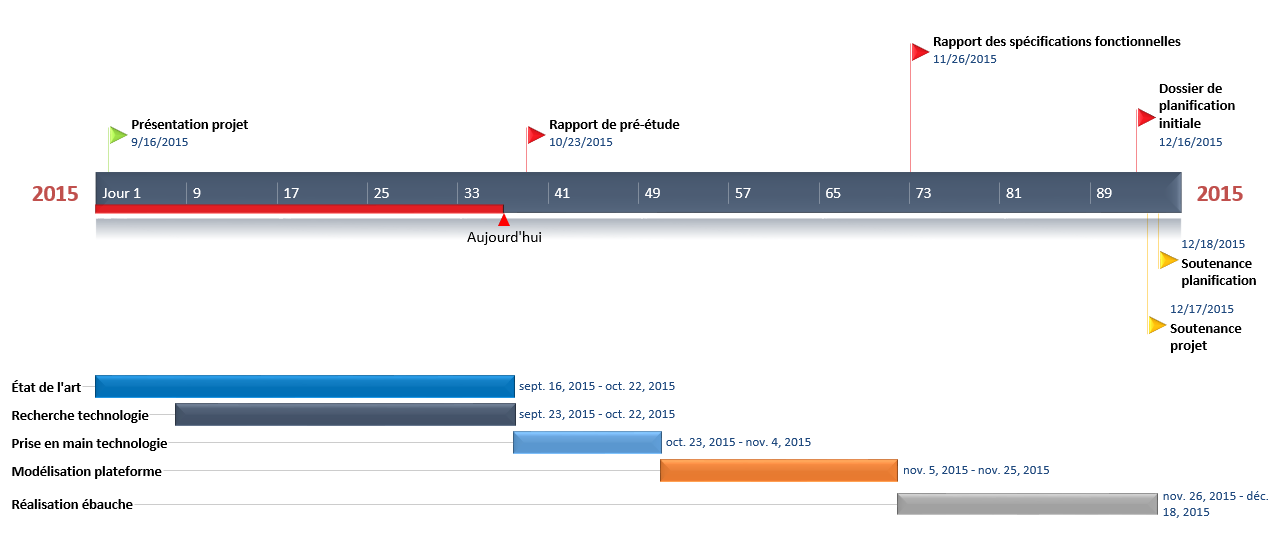
\includegraphics[width=1.3\textwidth, angle=90]{figure/timeline.png}
            \caption{Liste descriptive des tâches du planning d'analyse}
            \label{fig:description}
    \end{figure}

\section{Conclusion}
\label{Conclusion}
La numérisation de documents anciens est une problématique récente qui commence à toucher de plus en plus de
monde. Que ce soit par soucis de praticité ou de partage d’informations, on constate de plus en plus de sites
archivant de nombreux documents anciens, proposant plus ou moins de fonctionnalités. Certains sites sont d’ailleurs
consacrés spécifiquement à la presse ancienne, mais ceux-ci concernent les journaux provenant d’un pays et la plupart
ne sont accessibles que par abonnement.

Plusieurs plates-formes proposant des services similaires à ce que nous souhaitons proposer existent, ainsi un des
challenges de ce projet sera de pouvoir proposer toutes les fonctionnalités essentielles pour cette plate-forme,
et ce tout en offrant un service unique qui nous permettrait de nous démarquer des autres services.

Ainsi nous souhaitons proposer aux utilisateurs une plate-forme permettant de trouver efficacement et rapidement
tout journal présent dans notre base de données. Une navigation fluide et complète dans chaque journal permettra
de situer et trouver facilement des articles, des images ou du texte dans les pages de journaux qui peuvent atteindre
de très grandes tailles. Enfin nous aimerions proposer un espace collaboratif, où les utilisateurs pourront créer
des parcours thématiques regroupant des journaux ou articles autour d’un même évènement, qui seront ensuite proposés
aux lecteurs afin de naviguer entre des documents liés. Pour ce faire nous avons mis en avant plusieurs technologies
qui nous permettraient d’arriver à notre but.

Dans la suite du projet, nous allons nous pencher sur la faisabilité de toutes ces fonctionnalités dans le temps qui
nous est imparti et avec les ressources disponibles. Nous déciderons aussi précisément des tâches qui seront accomplies,
des technologies que nous utiliserons, et du planning de réalisation de l’application dans les futurs rapports.
